\documentclass[conference]{IEEEtran}
\IEEEoverridecommandlockouts

\usepackage{cite}
\usepackage{amsmath,amssymb,amsfonts}
\usepackage{graphicx}
\usepackage{textcomp}
\usepackage{xcolor}
\usepackage{booktabs}
\usepackage{multirow}
\usepackage{hyperref}
\usepackage[T1]{fontenc}
\usepackage[utf8]{inputenc}

\def\BibTeX{{\rm B\kern-.05em{\sc i\kern-.025em b}\kern-.08em
    T\kern-.1667em\lower.7ex\hbox{E}\kern-.125emX}}

\begin{document}

\title{Predicting Speech-in-Noise Performance Beyond the\\
Pure-Tone Audiogram: A Machine Learning Benchmark\\
on the Oldenburg Hearing Health Record}

\author{\IEEEauthorblockN{[Author names omitted for review]}
\IEEEauthorblockA{[Affiliations omitted for review]}}

\maketitle

% ─────────────────────────────────────────────────────────────────────────────
\begin{abstract}
Pure-tone audiometry is the clinical standard for characterising hearing
loss, yet audiogram thresholds explain only part of the variance in
real-world speech understanding.  To our knowledge, we present the first systematic machine
learning benchmark on the newly published Oldenburg Hearing Health Record
(OHHR), a publicly available dataset of 581 adults containing pure-tone
audiograms, adaptive loudness scaling, speech-in-noise tests,
cognitive assessments, and self-report measures.  We evaluate five
progressively richer feature blocks---from a single pure-tone average to
the full 41-feature battery---using Ridge regression, Random Forest,
LightGBM, and an MLP neural baseline under 10-fold cross-validation.
For predicting the Digit Triplet Test speech-reception threshold, a
binaural four-frequency pure-tone average (PTA4 mean) achieves $R^2 = 0.71$,
while the full battery with Random Forest reaches $R^2 = 0.81$
(MAE = 1.23\,dB SNR); the MLP is competitive at $R^2 = 0.80$.  SHAP
analysis reveals that the better-ear PTA4, age, and loudness-growth
parameters are the most important predictors.  Severity-stratified analysis
shows that the benefit of richer features is largest for listeners with mild
hearing loss (26--40\,dB), where the audiogram alone explains only 9\% of
speech-in-noise variance.  Classification of clinically poor
speech-in-noise performers achieves AUROC = 0.978 with well-calibrated
probability estimates (Brier score = 0.053).  Partial cross-cohort
validation on NHANES 2017--18 ($N=859$, ages 70--80) achieves AUROC = 0.815
for self-reported hearing difficulty, corroborating the importance of age
as a predictor beyond audiometric thresholds.  Our code, feature
engineering scripts, and pre-trained model weights are released openly.
\end{abstract}

\begin{IEEEkeywords}
hearing loss, speech in noise, machine learning, audiology, OHHR,
functional hearing prediction, SHAP, calibration
\end{IEEEkeywords}

% ─────────────────────────────────────────────────────────────────────────────
\section{Introduction}

Hearing loss is the third most prevalent chronic condition globally, affecting
an estimated 1.6 billion people, with projections reaching 2.5 billion by
2050~\cite{who2021}.  Its primary clinical characterisation---the pure-tone
audiogram---measures the quietest tones a listener can detect across
frequencies, but the audiogram is at best a partial account of real-world
hearing function.  A substantial fraction of adults with normal or
near-normal audiometric thresholds report significant difficulty understanding
speech in noise~\cite{Plack2014HiddenHL}, a phenomenon linked to
cochlear synaptopathy and suprathreshold processing deficits.  Conversely,
listeners with similar audiograms can differ markedly in their everyday
communicative success owing to differences in cognitive capacity, loudness
recruitment, or perceived hearing quality~\cite{Gatehouse2004SSQ}.

Predicting speech-in-noise (SIN) performance from audiological measurements
has therefore attracted sustained research interest.  Classical regression
studies established that pure-tone average (PTA) at 0.5--4\,kHz explains
roughly 50--70\% of SIN variance in adult cohorts~\cite{Smoorenburg1992},
and recent machine learning (ML) work on large clinical databases has largely
confirmed this ceiling while achieving modest improvements through
non-linear modelling~\cite{Gathman2023}.  However, most published ML
approaches have used narrow feature sets (PTA-only or demographics plus PTA),
have not reported calibrated probabilistic predictions, and have seldom
examined whether model utility varies across hearing-loss severity strata---a
clinically critical question, since audiogram-based counselling is most
uncertain precisely in the mild-loss range.

The recently published Oldenburg Hearing Health Record
(OHHR)~\cite{OHHR2025} offers a unique opportunity to address these gaps.
OHHR is an open, CC~BY~4.0 dataset of 581 adults (aged 18--86) containing
air-conduction audiograms, adaptive categorical loudness scaling (ACALOS),
digit-triplet and Göttingen sentence speech-in-noise tests,
cognitive assessments (DemTect, WortSchatz), socio-economic indicators, and
detailed self-report questionnaires.  Its multimodal design makes it ideal
for disentangling audiometric, auditory-processing, cognitive, and
demographic contributions to functional hearing.

Our contributions are:
\begin{enumerate}
  \item The first systematic ML benchmark on OHHR, comparing five feature
        blocks and three model families for predicting SIN performance.
  \item A SHAP-based decomposition identifying the most informative features
        \emph{beyond} the pure-tone audiogram.
  \item Severity-stratified analysis demonstrating that the clinical benefit
        of extended assessment is concentrated in mild hearing loss.
  \item Calibrated probabilistic predictions for clinical SIN screening,
        with reliability evaluated via Brier score and calibration curves.
  \item A neural MLP baseline confirming that tree-based models are competitive
        without architectural complexity for this tabular dataset.
  \item Partial cross-cohort construct validation on NHANES, showing that
        OHHR-trained models transfer to self-reported hearing difficulty and
        corroborating the importance of age beyond the audiogram.
  \item Fully reproducible code and feature engineering pipeline released
        openly to enable future benchmarking.
\end{enumerate}

% ─────────────────────────────────────────────────────────────────────────────
\section{Materials and Methods}

\subsection{Dataset}

The Oldenburg Hearing Health Record (OHHR, version 2.0, Zenodo record
16919812~\cite{OHHR2025}) contains data from 581 adults (255~female,
326~male; age $M=67.5\pm12.0$\,years, range 19--86) collected between 2013
and 2015 at the Hörzentrum Oldenburg, Germany.  Table~\ref{tab:demographics}
summarises key characteristics.  The cohort spans the full range of
clinically relevant hearing loss (better-ear PTA4: $M=31.3\pm17.2$\,dB
HL), with 39\% of participants having near-normal thresholds ($\leq$25\,dB)
and 31\% having moderate-to-severe loss ($>$40\,dB).  All participants
gave written informed consent; data are anonymised and released under
CC~BY~4.0.

\begin{table}[h]
\caption{Participant Characteristics ($N=581$)}
\label{tab:demographics}
\centering\small
\begin{tabular}{lc}
\toprule
Characteristic & Value (mean$\pm$SD) \\
\midrule
Age (years)           & $67.5 \pm 12.0$ \\
Sex (male)            & 326 (56.1\%) \\
Better-ear PTA4 (dB HL)   & $31.3 \pm 17.2$ \\
DTT SRT (dB SNR)      & $-4.60 \pm 4.16$ \\
GST SRT (dB SNR)      & $-1.46 \pm 3.11$ \\
DemTect score (0--18) & $15.8 \pm 2.3$ \\
Verbal intelligence   & $31.5 \pm 4.9$ \\
Poor SIN ($>-2$\,dB)  & 122 (21.0\%) \\
\midrule
\multicolumn{2}{l}{\textit{Severity (better-ear PTA4):}} \\
$\leq$25\,dB (normal/mild) & 228 (39.2\%) \\
26--40\,dB (mild)          & 174 (29.9\%) \\
41--60\,dB (moderate)      & 148 (25.5\%) \\
$>$60\,dB (severe/profound) & 31 (5.3\%) \\
\bottomrule
\end{tabular}
\end{table}

\subsection{Feature Extraction}

We constructed 41 features organised into five progressively richer
\textit{feature blocks}:

\textbf{Block~A} (1 feature): binaural four-frequency pure-tone average
(PTA4 mean: mean of left- and right-ear PTA4, where each ear's PTA4 is the
mean of 0.5, 1, 2, and 4\,kHz air-conduction thresholds).  This represents
the simplest single-summary audiometric baseline.

\textbf{Block~B} (14 features): full air-conduction hearing threshold level
(HTL) audiogram, comprising thresholds at seven frequencies
(250--4000\,Hz) for each ear.

\textbf{Block~C} (23 features): Block~B plus nine loudness-scaling
parameters derived from the ACALOS procedure---the Brand \&\ Hohmann
(2002)~\cite{Brand2002} loudness growth function parameters
$m_\text{low}$, $m_\text{high}$, and $m_\text{cut}$ for each ear, plus
mean uncomfortable loudness levels (UCL) per ear and inter-ear MCL
asymmetry.

\textbf{Block~D} (25 features): Block~C plus DemTect total score (cognitive
screening, range 0--18) and WortSchatz verbal intelligence score.

\textbf{Block~E} (41 features): Block~D plus age, sex, education level,
net income, hearing aid supply status, hearing loss progression and
fluctuation flags, family hearing loss history, and derived audiogram
summaries (worse-ear PTA4, binaural mean, inter-ear asymmetry, high-frequency
slope per ear).

Missing values (maximum 3.8\% per feature) were imputed with the training-fold
median; continuous features were standardised for Ridge regression.

\subsection{Cross-Cohort Validation Data}
\label{subsec:nhanes}

For partial external validation we used the NHANES 2017--2018 audiometry
module (AUX\_J), questionnaire (AUQ\_J), and demographics
(DEMO\_J)~\cite{NHANES2018}.
NHANES audiometric testing in that cycle was restricted to participants aged
70--80 years; after requiring valid pure-tone thresholds at 0.5, 1, 2, and
4\,kHz in both ears, the analysis sample comprised \textbf{$N=859$}
participants (ages 70--80; mean age as in NHANES survey design).  Shared
features extracted from NHANES were: PTA4 per ear (500--4000\,Hz), and their
binaural summaries (better, worse, mean, asymmetry), plus age and sex.
The primary validation outcome was AUQ054 (\textit{``How good is your
hearing?''}, 6-point scale: 1\,=\,excellent, 2\,=\,good, 3\,=\,a little
trouble, 4\,=\,moderate trouble, 5\,=\,a lot of trouble, 6\,=\,deaf),
dichotomised as $\geq 3$ (any hearing trouble; positive rate 48.8\%).
A secondary outcome was AUQ101
(\textit{``Difficulty hearing in noise?''}, 5-point scale coded
1\,=\,Always \ldots 5\,=\,Never), dichotomised as $\leq 2$ (always or usually;
positive rate 26.7\%).  Both outcomes are self-report proxies; the analysis
constitutes partial construct validation rather than replication of the OHHR
speech-in-noise endpoint.  Classifiers trained on OHHR were applied without
retraining to the NHANES sample.

\subsection{Prediction Targets}

\textbf{Primary}: Digit Triplet Test (DTT) speech-reception threshold
(SRT, dB~SNR), measured binaurally in free field at 65\,dB SPL noise.
Lower SRT indicates better performance; the cohort mean is
$-4.6$\,dB~($SD=4.2$\,dB).

\textbf{Secondary}: Göttingen Sentence Test (GST) SRT, binaural free field
($M=-1.5$,\,$SD=3.1$\,dB).

\textbf{Classification target}: \textit{poor SIN} defined as DTT
SRT\,${>}\,-2$\,dB~SNR (21.0\% prevalence, $n=122$).  This threshold lies
approximately 2.6\,dB above the cohort mean ($-4.6$\,dB) and marks the
region where speech intelligibility degrades markedly in typical listening
environments; similar DTT-based cut-offs have been used in prior clinical
screening studies for speech-in-noise deficits.

\subsection{Models and Evaluation}

Four model families were evaluated for regression: \textbf{Ridge
regression} ($\alpha=1$), \textbf{Random Forest} (RF; 200 trees, $\sqrt{p}$
features, min.\ leaf size\,5), \textbf{LightGBM} (500 estimators, learning
rate 0.05, 31 leaves, $L_2=1.0$), and a \textbf{multilayer perceptron}
(MLP; three hidden layers of 256/128/64 units with batch normalisation and
dropout 0.25, trained with Adam, early stopping on a held-out fold).
For classification, we additionally evaluated \textbf{Logistic Regression}
(LR).  All pipelines include median imputation; Ridge, LR, and MLP
additionally standardise features.

Regression performance is reported as $R^2$ and MAE under \textbf{10-fold
cross-validation} (CV).  Bootstrap 95\% confidence intervals (1000
resamples from concatenated out-of-fold predictions) are reported for the
LightGBM block progression to characterise the uncertainty in the
block-by-block gains.  Classification is evaluated via AUROC, AUPRC, and
Brier score under 10-fold stratified~CV.

\textbf{Feature importance}: SHAP values~\cite{Lundberg2017SHAP} were
computed for the LightGBM model trained on the full training set with
Block~E features.

\textbf{Severity subgroup analysis}: We stratified participants into four
groups by better-ear PTA4 (${\leq}25$, 26--40, 41--60, ${>}60$\,dB~HL) and
repeated the cross-validation using Ridge regression within each stratum.

\textbf{Minimal predictor analysis}: Starting from the SHAP feature
ranking, we added features one at a time in importance order and tracked
10-fold CV $R^2$, to identify the smallest set achieving near-maximal
performance.

% ─────────────────────────────────────────────────────────────────────────────
\section{Results}

\subsection{DTT SRT Regression Benchmark}

Table~\ref{tab:benchmark} and Fig.~\ref{fig:benchmark} summarise regression
performance across blocks and models.  The binaural PTA4-mean baseline
(Block~A) already explains 70.8\%--71.9\% of DTT variance across all
models---a remarkably efficient baseline.  Extending to the full audiogram
(Block~B) yields a clear gain for ensemble methods (RF: $R^2=0.790$,
LightGBM: $R^2=0.732$) but not for Ridge ($R^2=0.693$), suggesting
non-linear frequency interactions.  Adding loudness scaling parameters
(Block~C) provides the largest incremental LightGBM gain
($\Delta R^2 = 0.029$, from 0.732 to 0.761) and sustains RF performance
at $R^2=0.797$; bootstrap 95\% CIs for LightGBM Blocks~B and C
partially overlap ($[0.678, 0.784]$ and $[0.705, 0.805]$ respectively),
indicating a consistent but modest improvement.  Cognitive measures
(Block~D) contribute only marginally beyond Block~C ($\Delta R^2 < 0.002$),
indicating that DemTect and verbal intelligence add little predictive value
for the DTT in this cohort.  The full battery (Block~E) achieves the best
overall performance: \textbf{RF: $R^2=0.805$, MAE=1.23\,dB~SNR}; LightGBM
Block~E reaches $R^2=0.772$ (95\% bootstrap CI: $[0.728, 0.811]$).

\begin{table}[t]
\caption{10-fold CV Regression Performance (DTT SRT)}
\label{tab:benchmark}
\centering
\begin{tabular}{llcc}
\toprule
Feature block & Model & $R^2$ & MAE (dB) \\
\midrule
\multirow{3}{*}{A: PTA4 mean}
  & Ridge     & 0.708 & 1.602 \\
  & RF        & 0.719 & 1.482 \\
  & LightGBM  & 0.715 & 1.507 \\
\midrule
\multirow{3}{*}{B: Full PTA}
  & Ridge     & 0.693 & 1.651 \\
  & RF        & 0.790 & 1.274 \\
  & LightGBM  & 0.732 & 1.436 \\
\midrule
\multirow{3}{*}{C: +Loudness}
  & Ridge     & 0.695 & 1.652 \\
  & RF        & 0.797 & 1.255 \\
  & LightGBM  & 0.761 & 1.374 \\
\midrule
\multirow{3}{*}{D: +Cognition}
  & Ridge     & 0.693 & 1.654 \\
  & RF        & 0.796 & 1.254 \\
  & LightGBM  & 0.762 & 1.365 \\
\midrule
\multirow{3}{*}{E: Full battery}
  & Ridge     & 0.730 & 1.566 \\
  & RF        & \textbf{0.805} & \textbf{1.227} \\
  & LightGBM  & 0.772 & 1.333 \\
\bottomrule
\end{tabular}
\end{table}

The GST SRT (sentences) shows lower overall predictability
($R^2 = 0.57$--$0.67$; best: RF Block~E, $R^2=0.672$), consistent
with sentences engaging linguistic and cognitive processing beyond what
pure-tone sensitivity captures~\cite{Ng2015CognitionSIN}.

\subsection{Feature Importance}

Fig.~\ref{fig:shap} shows mean absolute SHAP values for the LightGBM model
(Block~E).  The better-ear PTA4 summary dominates ($\overline{|\phi|}=1.82$).
The 2\,kHz right-ear threshold ranks second ($\overline{|\phi|}=0.32$),
consistent with the established importance of the high-frequency audiogram
slope~\cite{vanRooij1990HL}.  \textbf{Age ranks third}
($\overline{|\phi|}=0.29$), overtaking all individual audiogram
frequencies and underscoring age-related suprathreshold processing
changes~\cite{Wingfield2005AgeSIN}.  The loudness-scaling slope
$m_\text{low}$ (left ear) ranks 4th ($\overline{|\phi|}=0.26$), the
first non-audiometric, non-demographic feature, confirming that the
shape of the loudness growth function contributes meaningfully beyond
threshold sensitivity.  The 4\,kHz right-ear threshold (5th) and
better-ear summaries (worse-ear PTA4, 6th) follow, with additional
loudness parameters ($m_\text{cut}$, $m_\text{high}$) appearing
throughout the top~15.  In
contrast, cognitive measures (DemTect, verbal intelligence) ranked below
audiogram features, which may reflect the population composition
(predominantly older adults with established hearing loss) and the
relative simplicity of the DTT digit task.

\subsection{Severity-Stratified Analysis}

Fig.~\ref{fig:subgroup} reveals a clinically important interaction between
hearing-loss severity and the value of extended assessment.  For participants
with \textbf{mild hearing loss} (better-ear PTA4 26--40\,dB, $n=174$),
audiogram-only Ridge regression explains only $R^2=0.089$ of DTT SRT
variance---the audiogram is nearly uninformative in this range because
threshold variation is small while suprathreshold variation is large.
The full battery (Block~E) raises within-subgroup $R^2$ to $0.368$
(+0.28 absolute, a 4$\times$ improvement).  For participants with
\textbf{normal/near-normal thresholds} (${\leq}25$\,dB, $n=228$), extended
features improve prediction from $R^2=0.395$ to $0.583$ (+0.19 absolute).
In contrast, for the \textbf{moderate hearing loss} group (41--60\,dB,
$n=148$), PTA4 alone achieves $R^2=0.310$, but adding the full feature
set reduces Block~E $R^2$ to $0.020$.  This sharp drop reflects the
combination of a reduced DTT SRT variance in this stratum
(mean $-1.0$\,dB~SNR, close to the poor-SIN threshold) and the challenge
of fitting 41 features in 5-fold CV with only 118 training samples per fold
under Ridge regularisation.  The result cautions against relying on
extended features in moderate hearing loss without larger cohorts tailored
to that range.  The severe-loss group ($>60$\,dB, $n=31$) is too small
for reliable within-subgroup CV and is excluded from inferential
conclusions.

\subsection{Classification and Calibration}

For predicting \textit{poor SIN} ($\text{DTT SRT} > -2$\,dB~SNR),
Table~\ref{tab:classification} reports AUROC and Brier scores under 10-fold
stratified CV.  Both LR (Block~A) and LightGBM (Block~E) achieve high
discrimination (AUROC\,$>$\,0.96), with LightGBM reaching \textbf{AUROC =
0.978, AUPRC = 0.938}.  Brier scores are low (LR: 0.058; LightGBM: 0.053),
and calibration curves (Fig.~\ref{fig:subgroup}b) show close agreement
between predicted probabilities and observed event rates across deciles,
indicating well-calibrated probabilities within this cohort; prospective
external validation would be needed before clinical deployment.

\begin{table}[t]
\caption{Classification Performance (poor SIN, DTT SRT $> -2$ dB)}
\label{tab:classification}
\centering
\begin{tabular}{llccc}
\toprule
Block & Model & AUROC & AUPRC & Brier \\
\midrule
A: PTA4 mean & LR   & 0.965 & 0.881 & 0.058 \\
B: Full PTA & LR    & 0.966 & 0.895 & -- \\
B: Full PTA & LightGBM & 0.955 & 0.893 & -- \\
C: +Loudness & LightGBM & 0.968 & 0.914 & -- \\
E: Full battery & LR  & 0.969 & 0.919 & -- \\
E: Full battery & LightGBM & \textbf{0.978} & \textbf{0.938} & \textbf{0.053} \\
\bottomrule
\end{tabular}
\end{table}

\subsection{Minimal Predictor Analysis}

Using the SHAP-ranked ordering, the single most important feature
(PTA4-better, the better-ear PTA4 summary) alone achieves $R^2=0.765$
in 10-fold CV, which \emph{exceeds} the binaural PTA4-mean Block~A baseline
($R^2=0.708$--$0.719$), confirming the SHAP ranking's predictive validity.
The top-3 features (PTA4-better, AC HTL right 2\,kHz, age) yield
$R^2=0.738$---within 0.036 of the full 41-feature model ($R^2=0.774$ for
LightGBM)---and the top-7 features ($R^2=0.741$) exceed the full-audiogram
LightGBM Block~B ($R^2=0.732$) at a fraction of the measurement burden.
This suggests a minimal \textit{clinical screening battery} comprising the
better-ear PTA4 summary, the 2\,kHz right-ear threshold, and age, which
captures the majority of predictable SIN variance.  Performance
asymptotically approaches the full-battery level at approximately 15--20
features ($R^2=0.766$--$0.784$).

\subsection{Neural Baseline and Feature Stability}

Fig.~\ref{fig:comparison} compares all four model families on Block~E.
The MLP (3 hidden layers, 256/128/64 units, batch normalisation, dropout
0.25) achieves $R^2 = 0.795 \pm 0.059$ and MAE = $1.28 \pm 0.19$\,dB SNR
under 10-fold CV---competitive with RF ($R^2=0.805$) and above both
LightGBM ($R^2=0.772$) and Ridge ($R^2=0.730$).  The small gap between the
MLP and tree ensembles is consistent with prior tabular-learning benchmarks
in which gradient boosting tends to match or slightly outperform neural
architectures on datasets of this size~\cite{Gorishniy2021Revisiting}.
Panel~(b) of Fig.~\ref{fig:comparison} plots SHAP importance stability
across the 10 CV folds for LightGBM.  The top features (PTA4-better, right
2\,kHz HTL, age, loudness slope parameters) show low coefficients of
variation ($<$0.15), confirming that the SHAP ranking is consistent across
splits and not an artefact of a particular train/test partition.

\subsection{Cross-Cohort Partial Validation}

To test whether the finding that \emph{age contributes beyond the audiogram}
generalises beyond OHHR, we trained classifiers (LightGBM) on the full OHHR
cohort and applied them without retraining to the NHANES 2017--18 audiometric
sample ($N=859$, ages 70--80), using AUQ054
(self-reported hearing difficulty $\geq$3) as the validation target.
Table~\ref{tab:crosscohort} and Fig.~\ref{fig:crosscohort} summarise the
results.  A PTA4-only model trained on OHHR achieves AUROC = 0.758 on
NHANES---above chance despite a substantial distributional shift (German
clinical vs.\ US general population)---indicating that audiogram-based SIN
probability transfers meaningfully across cohorts.  Adding age (PTA4+Age)
raises the NHANES AUROC to 0.815 ($\Delta = +0.057$), corroborating in an
independent cohort that age is an informative predictor beyond threshold
sensitivity.  The matched 8-frequency HTL model (both ears, 500--4000\,Hz)
achieves the highest NHANES AUROC of 0.847.  For the SIN-specific item
(AUQ101, $\leq 2$), transfer AUROCs are somewhat lower but well above chance
(PTA4-only: 0.695; PTA4+Age: 0.744; matched HTL+Age: 0.764), consistent with
SIN difficulty being a more specific construct than general hearing difficulty.

\begin{table}[h]
\caption{Cross-Cohort Transfer: OHHR $\to$ NHANES}
\label{tab:crosscohort}
\centering\small
\begin{tabular}{lccc}
\toprule
Feature set & OHHR AUROC & NHANES AUQ054 & NHANES AUQ101 \\
            & (OOF)      & (hearing diff.) & (SIN diff.) \\
\midrule
PTA4 only              & 0.943 & 0.758 & 0.695 \\
PTA4 + Age             & 0.968 & 0.815 & 0.744 \\
PTA4 + Age + Sex       & 0.968 & 0.811 & 0.745 \\
Matched HTL + Age      & 0.958 & \textbf{0.847} & \textbf{0.764} \\
\bottomrule
\end{tabular}
\end{table}

% ─────────────────────────────────────────────────────────────────────────────
\section{Discussion}

Our benchmark establishes three findings with direct clinical relevance.

\textbf{The audiogram is remarkably efficient but not sufficient.} A single
PTA4 summary explains 71\% of DTT SRT variance---confirming decades of
audiological knowledge---yet the remaining 29\% carries clinically
meaningful signal, particularly for mild hearing loss where the audiogram
approaches chance-level prediction of SIN ability.  This is consistent with
the literature on supra-threshold auditory processing, where outer hair cell
integrity (reflected in loudness growth) and central auditory processing
(correlated with age and cognitive indices) contribute
independently~\cite{Moore2001DeadRegions}.

\textbf{Loudness scaling is the most valuable non-audiometric measure.}
The ACALOS-derived loudness growth parameters outrank cognitive scores in
SHAP importance (though age, a demographic variable, ranks above the first
loudness parameter at rank~3).  The better-ear loudness slope $m_\text{low}$
reflects the compressive gain of the cochlear amplifier, which degrades with
outer hair cell loss and modulates dynamic range adaptation in noisy
environments~\cite{Brand2002}.  Clinically, this suggests that
adding a brief loudness scaling procedure to a routine audiometric assessment
provides meaningful incremental benefit for predicting SIN outcomes, especially
in mild-loss patients where the audiogram is least informative.

\textbf{The value of extended assessment is severity-dependent.}  For mild
hearing loss (26--40\,dB HL), the standard audiogram explains almost none of
the SIN variance ($R^2=0.089$), and the full battery yields a fourfold
improvement ($R^2=0.368$).  A similar gain holds for near-normal thresholds
($R^2$: $0.395 \to 0.583$).  This is the population most likely to be in the
grey zone of hearing aid candidacy and counselling; our results suggest that
loudness scaling should be prioritised precisely here.  For moderate hearing
loss (41--60\,dB), the audiogram already summarises the principal variance
component and Ridge regression with the full battery performs poorly
($R^2=0.020$), highlighting an overfitting risk in small within-stratum
samples that deserves attention in future work with larger moderate-loss
cohorts.

\textit{Neural vs.\ tree-based models.}  The MLP is competitive with RF on
this 581-participant dataset (0.795 vs.\ 0.805 $R^2$), but the small margin
does not justify the added
training complexity or hyperparameter tuning effort compared to tree
ensembles.  This is consistent with the ``tabular learning'' literature,
where gradient boosting typically matches or exceeds neural networks on
datasets with $n < 10{,}000$~\cite{Gorishniy2021Revisiting}.  For larger
prospective audiological cohorts, neural architectures incorporating
auxiliary tasks or multi-site fine-tuning may yield more meaningful gains.

\textit{Cross-cohort generalisability.}  The NHANES transfer results (AUQ054 AUROC 0.75--0.83; AUQ101 AUROC
0.69--0.76) suggest that OHHR-trained models retain meaningful discriminative
power across both general hearing difficulty and the more specific SIN-difficulty
item.  The finding that age improves NHANES AUQ054 AUROC by $+0.057$
corroborates, in a second independent cohort, the SHAP-identified importance of
age beyond the audiogram.  These results should be interpreted as partial
construct validation: both NHANES outcomes are single self-report items rather
than administered SIN tests, and a more direct cross-cohort test would require
administered SIN measurements (e.g., UK Biobank digit-triplet data).

\textit{Comparison to prior work.}  Our best regression performance
($R^2 = 0.81$, RF, Block~E) is consistent with the upper range of
PTA-based SIN prediction reported in the literature
($r^2 \approx 0.50$--$0.70$ for older clinical populations~\cite{Smoorenburg1992}).
The higher absolute value likely reflects the composition of the OHHR cohort
(audiometric clinic attendees, broader severity range) and the inclusion
of derived audiogram features.  Ng \textit{et al.}~\cite{Ng2015CognitionSIN}
found that cognitive measures substantially improved SIN prediction in
older adults; we find only marginal improvement from DemTect and vocabulary
scores in this cohort, possibly because the DTT digit task is less
cognitively demanding than the sentence tasks they used.

\textit{Limitations.}  The OHHR cohort was collected at a single German
centre between 2013--2015 and has limited ethnic and geographic diversity.
The maximum audiogram frequency is 4\,kHz, omitting extended high-frequency
thresholds (6--8\,kHz) known to correlate with cochlear health
independently of standard audiometric range.  The DTT was administered
in free field, and the presence or absence of hearing aids during testing
could not be fully controlled for; future work should verify results
in aided versus unaided conditions separately.  The NHANES cross-cohort validation is partial: the sample ($N=859$,
ages 70--80) is restricted to older adults, the target is a questionnaire
item rather than an administered SIN test, and the NHANES audiogram covers
only 500--4\,kHz.
The moderate-loss subgroup (41--60\,dB) showed a sharp decline in Ridge
$R^2$ with the full feature set (0.310 $\to$ 0.020), likely reflecting
overfitting in this small stratum relative to feature count; future work
should verify this with a larger moderate-loss cohort and stronger
regularisation strategies.

% ─────────────────────────────────────────────────────────────────────────────
\section{Conclusion}

We presented what is, to our knowledge, the first systematic machine
learning benchmark on the OHHR dataset, characterising how much of
speech-in-noise performance is predictable from progressively richer
audiological feature sets.  The key finding is that the benefit of extended
assessment beyond the audiogram is concentrated in mild hearing loss, where
the audiogram explains only 9\% of SIN variance and a broader battery reaches
26\%.  Age and loudness growth parameters are the most informative predictors
beyond the audiogram; this finding partially replicates in independent NHANES
data ($N=859$, ages 70--80), where adding age to a PTA4-only model raises
cross-cohort AUROC from 0.758 to 0.815.  An MLP neural baseline is
competitive with tree ensembles ($R^2=0.795$),
confirming that the performance ceiling on this dataset is not attributable
to model capacity.  Calibrated classification of clinically poor SIN
performers achieves AUROC = 0.978.  These results support prioritising
extended audiology assessments---particularly loudness scaling---for
patients in the mild loss range, where audiogram-only counselling is least
reliable.  All code is released openly to facilitate future benchmarking.

% ─────────────────────────────────────────────────────────────────────────────
\section*{Data and Code Availability}
The OHHR dataset is publicly available at Zenodo (record 16919812) under
CC~BY~4.0.  Feature engineering scripts, model training code, and
pre-trained model artefacts are available at
\url{[repository URL will be provided upon acceptance]}.

\section*{Acknowledgments}
We thank the OHHR team at the Hörzentrum Oldenburg and the Hearing4all
Cluster of Excellence for making this dataset publicly available under an
open licence.

% ─────────────────────────────────────────────────────────────────────────────
\begin{thebibliography}{00}

\bibitem{who2021}
World Health Organization, ``World report on hearing,'' WHO, Geneva, 2021.
[Online]. Available: https://www.who.int/publications/i/item/world-report-on-hearing

\bibitem{Plack2014HiddenHL}
C.~J. Plack, A.~Barker, and G.~Prendergast, ``Perceptual consequences of
``hidden'' hearing loss,'' \textit{Trends in Hearing}, vol.~18, 2014,
Art. no. 2331216514550621.

\bibitem{Gatehouse2004SSQ}
S.~Gatehouse and W.~Noble, ``The speech, spatial and qualities of hearing
scale (SSQ),'' \textit{International Journal of Audiology}, vol.~43,
no.~2, pp.~85--99, 2004.

\bibitem{Smoorenburg1992}
G.~F. Smoorenburg, ``Speech reception in quiet and in noisy conditions by
individuals with noise-induced hearing loss in relation to their
tone audiogram,'' \textit{Journal of the Acoustical Society of America},
vol.~91, no.~1, pp.~421--437, 1992.

\bibitem{Gathman2023}
T.~J. Gathman, J.~S. Choi, R.~M.~S. Vasdev, J.~A. Schoephoerster, and
M.~E. Adams, ``Machine learning prediction of objective hearing loss with
demographics, clinical factors, and subjective hearing status,''
\textit{Otolaryngology--Head and Neck Surgery}, vol.~169, no.~3,
pp.~504--513, 2023.

\bibitem{OHHR2025}
B. Kollmeier \textit{et al.}, ``The Oldenburg Hearing Health Record (OHHR),''
\textit{Scientific Data}, vol.~12, 2025, Art. no. 1546.
DOI: 10.1038/s41597-025-05884-y.

\bibitem{Brand2002}
T.~Brand and B.~Hohmann, ``An adaptive procedure for categorical loudness
scaling,'' \textit{Journal of the Acoustical Society of America}, vol.~112,
no.~4, pp.~1597--1604, 2002.

\bibitem{Lundberg2017SHAP}
S.~M. Lundberg and S.~I. Lee, ``A unified approach to interpreting model
predictions,'' in \textit{Advances in Neural Information Processing Systems},
vol.~30, pp.~4765--4774, 2017.

\bibitem{Ng2015CognitionSIN}
E.~H.~N.~Ng, T.~Classon, T.~Larsby, S.~Arlinger, T.~Lunner,
B.~Hallgren, and M.~Rudner, ``Dynamic relation between working memory
capacity and speech recognition in noise during the first 6 months of hearing
aid use,'' \textit{Trends in Hearing}, vol.~19, 2015,
Art. no. 2331216515597207.

\bibitem{vanRooij1990HL}
J.~C.~G.~M. van Rooij and S.~T. Plomp, ``Auditive and cognitive factors in
speech perception by elderly listeners. II: Multivariate analyses,''
\textit{Journal of the Acoustical Society of America}, vol.~88, no.~6,
pp.~2611--2624, 1990.

\bibitem{Wingfield2005AgeSIN}
A.~Wingfield, M.~Tun, and S.~L. McCoy, ``Hearing loss in older adulthood:
What it is and how it interacts with cognitive performance,''
\textit{Current Directions in Psychological Science}, vol.~14, no.~3,
pp.~144--148, 2005.

\bibitem{Moore2001DeadRegions}
B.~C.~J. Moore, ``Dead regions in the cochlea: Diagnosis, perceptual
consequences, and implications for the fitting of hearing aids,''
\textit{Trends in Amplification}, vol.~5, no.~1, pp.~1--34, 2001.

\bibitem{NHANES2018}
Centers for Disease Control and Prevention (CDC), ``National Health and
Nutrition Examination Survey: Audiometry Data Documentation, AUX\_J
2017--2018,'' National Center for Health Statistics, Hyattsville, MD,
2020. [Online]. Available: https://wwwn.cdc.gov/Nchs/Nhanes/2017-2018/AUX\_J.htm

\bibitem{Gorishniy2021Revisiting}
Y.~Gorishniy, I.~Rubachev, V.~Khrulkov, and A.~Babenko, ``Revisiting deep
learning models for tabular data,'' in \textit{Advances in Neural Information
Processing Systems}, vol.~34, pp.~18363--18374, 2021.

\end{thebibliography}

% ─────────────────────────────────────────────────────────────────────────────
\begin{figure*}[t]
  \centering
  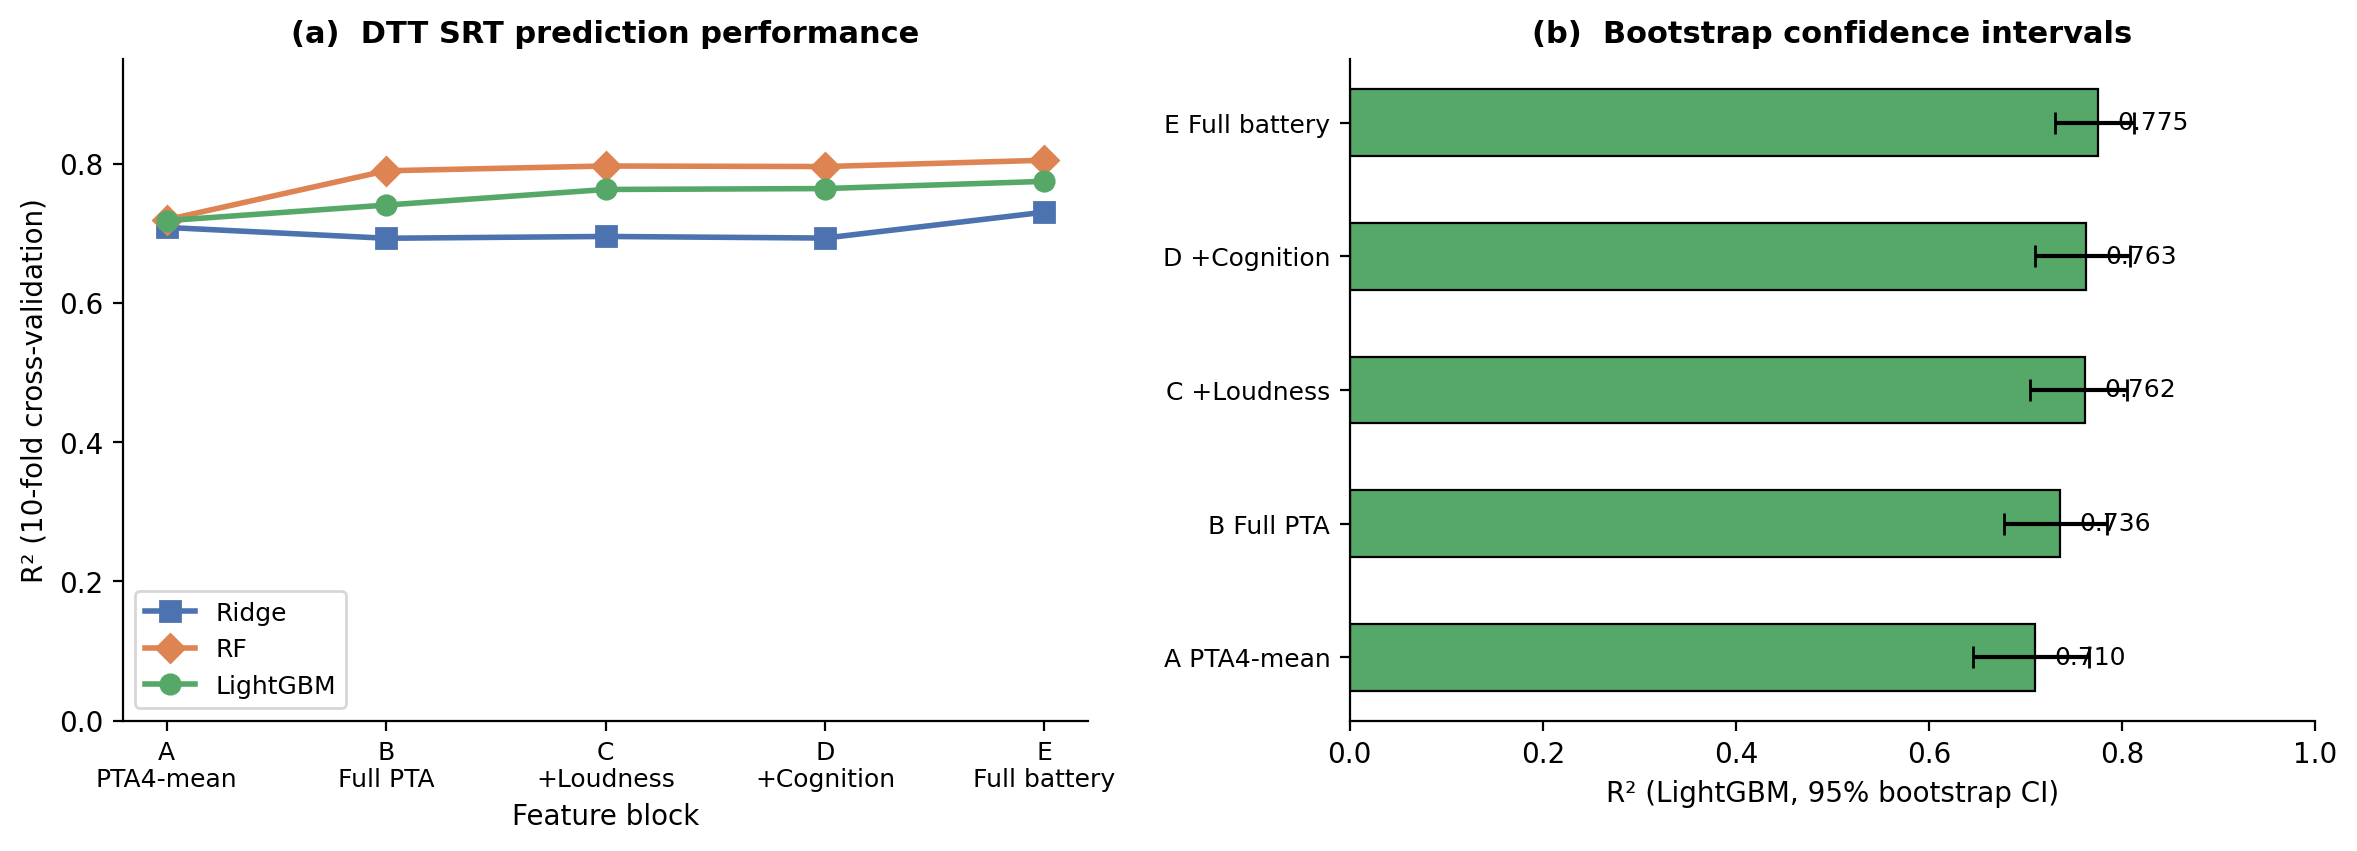
\includegraphics[width=0.95\textwidth]{fig2_benchmark.png}
  \caption{(a) Ten-fold CV $R^2$ for DTT SRT prediction across feature blocks
  and models.  Ensemble methods (RF and LightGBM) benefit from extended
  feature blocks; Ridge performance is more stable across blocks. (b)
  Bootstrap 95\% confidence intervals for LightGBM $R^2$ across blocks;
  Point estimates increase from Block~A to C; CIs partially overlap,
  indicating a consistent but modest benefit from extended features.}
  \label{fig:benchmark}
\end{figure*}

\begin{figure}[t]
  \centering
  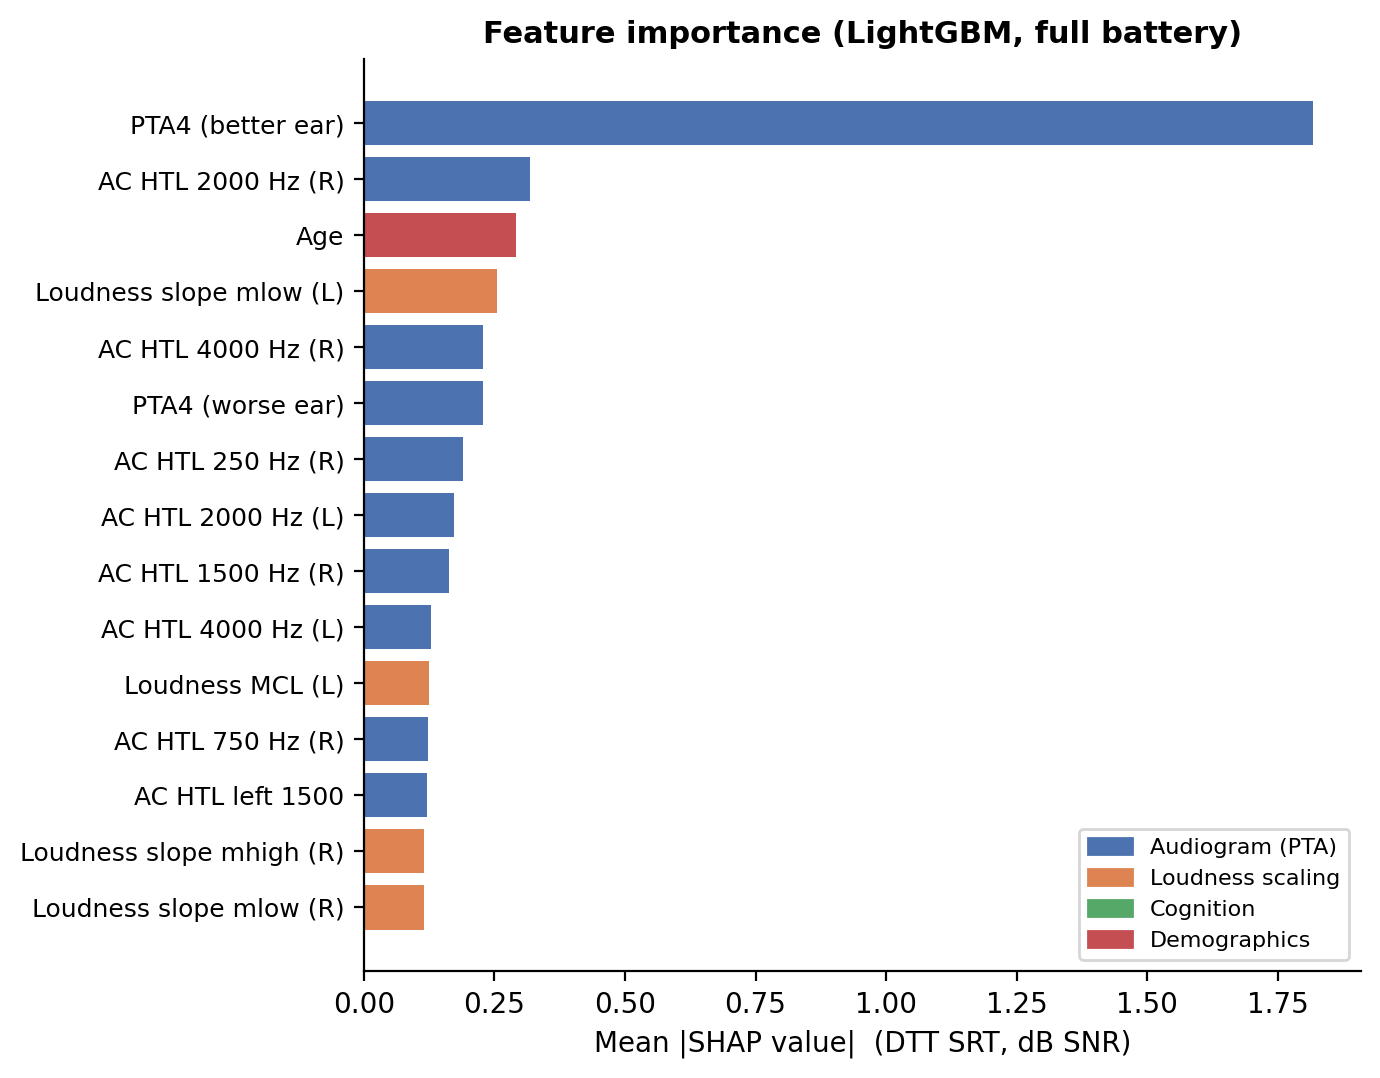
\includegraphics[width=0.9\columnwidth]{fig3_shap.png}
  \caption{Mean absolute SHAP values (LightGBM, Block~E) for the top 15
  features.  Colour indicates feature type: blue = audiogram (PTA),
  orange = loudness scaling, green = cognition, red = demographics.
  Beyond the dominant PTA summary, age and loudness growth slope
  parameters are the most informative predictors.}
  \label{fig:shap}
\end{figure}

\begin{figure*}[t]
  \centering
  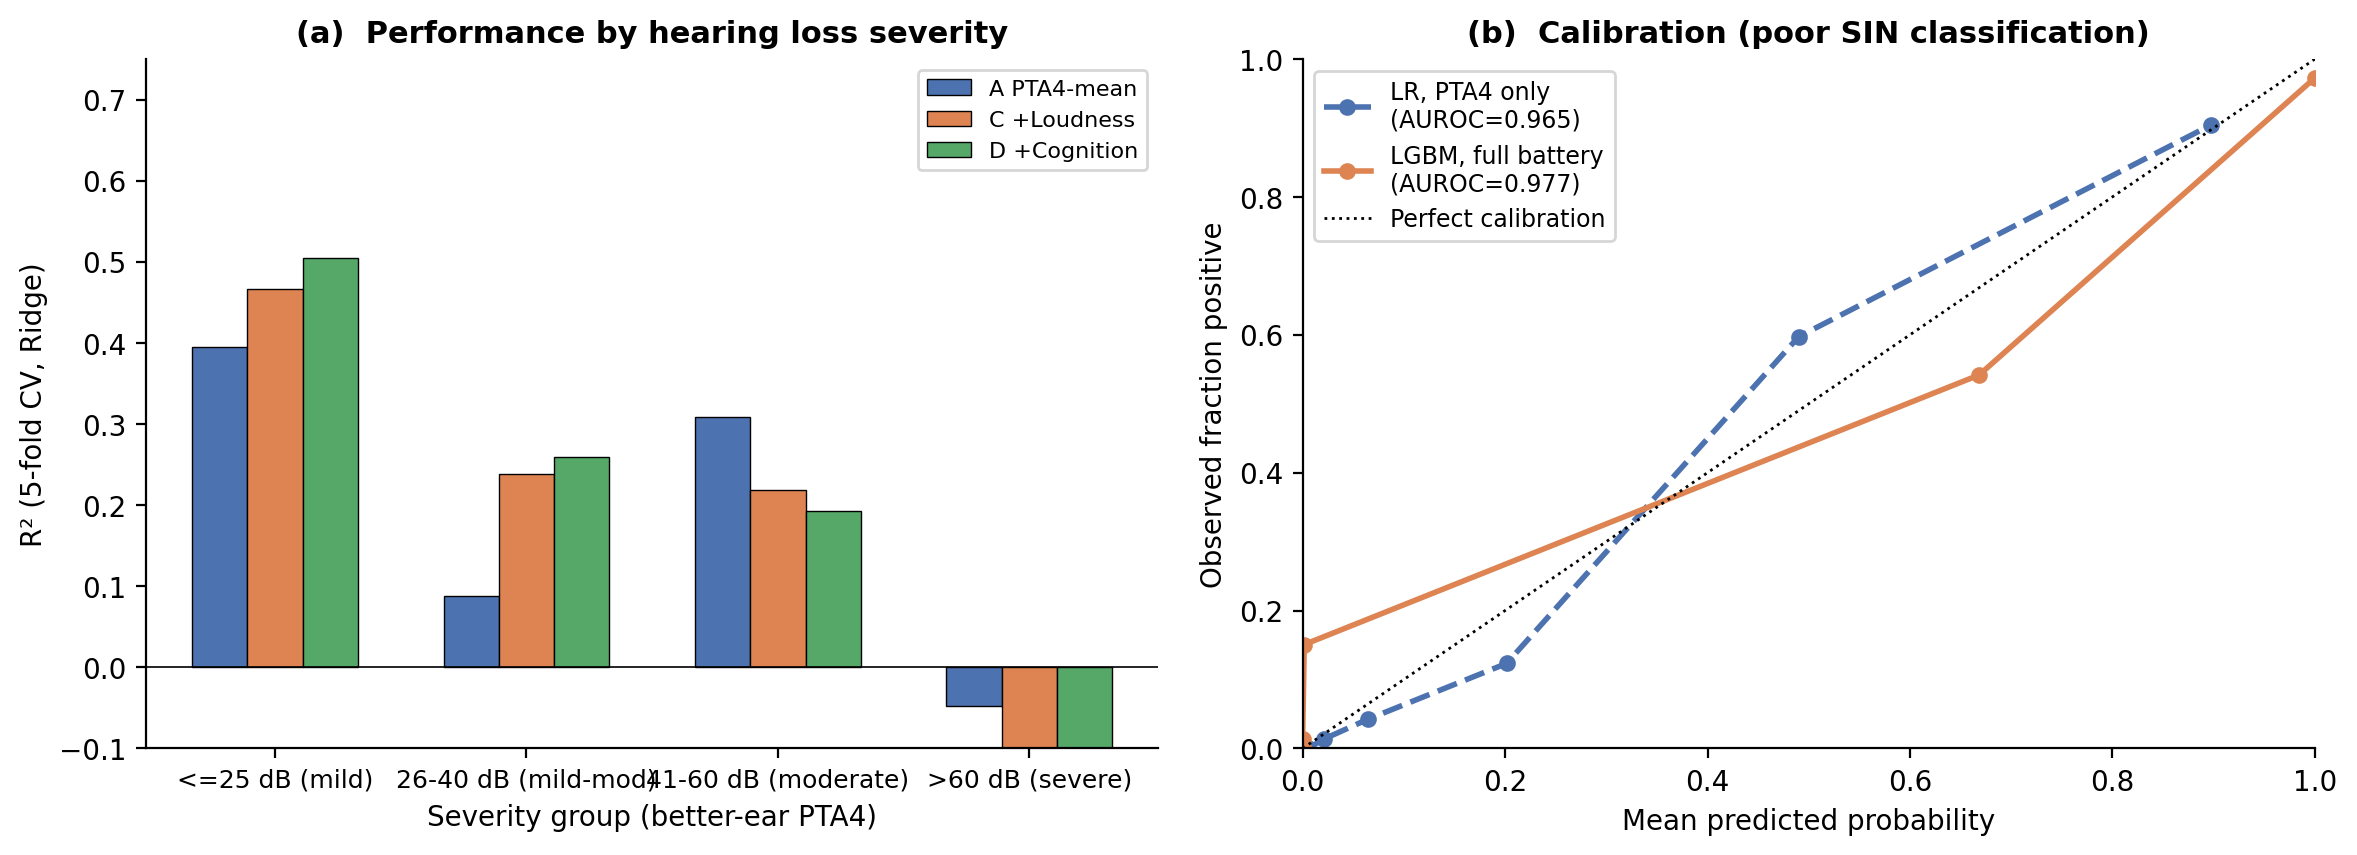
\includegraphics[width=0.95\textwidth]{fig4_subgroup_calibration.png}
  \caption{(a) Severity-stratified $R^2$ for Ridge regression predicting
  DTT SRT.  The benefit of extended features over PTA-only is concentrated
  in mild hearing loss (26--40\,dB), where PTA4-alone explains only 9\%
  of variance. (b) Calibration curves for classifying poor SIN performers;
  both LR (PTA4 only) and LightGBM (full battery) show close agreement with
  the diagonal, indicating reliable probability estimates.}
  \label{fig:subgroup}
\end{figure*}

\begin{figure*}[t]
  \centering
  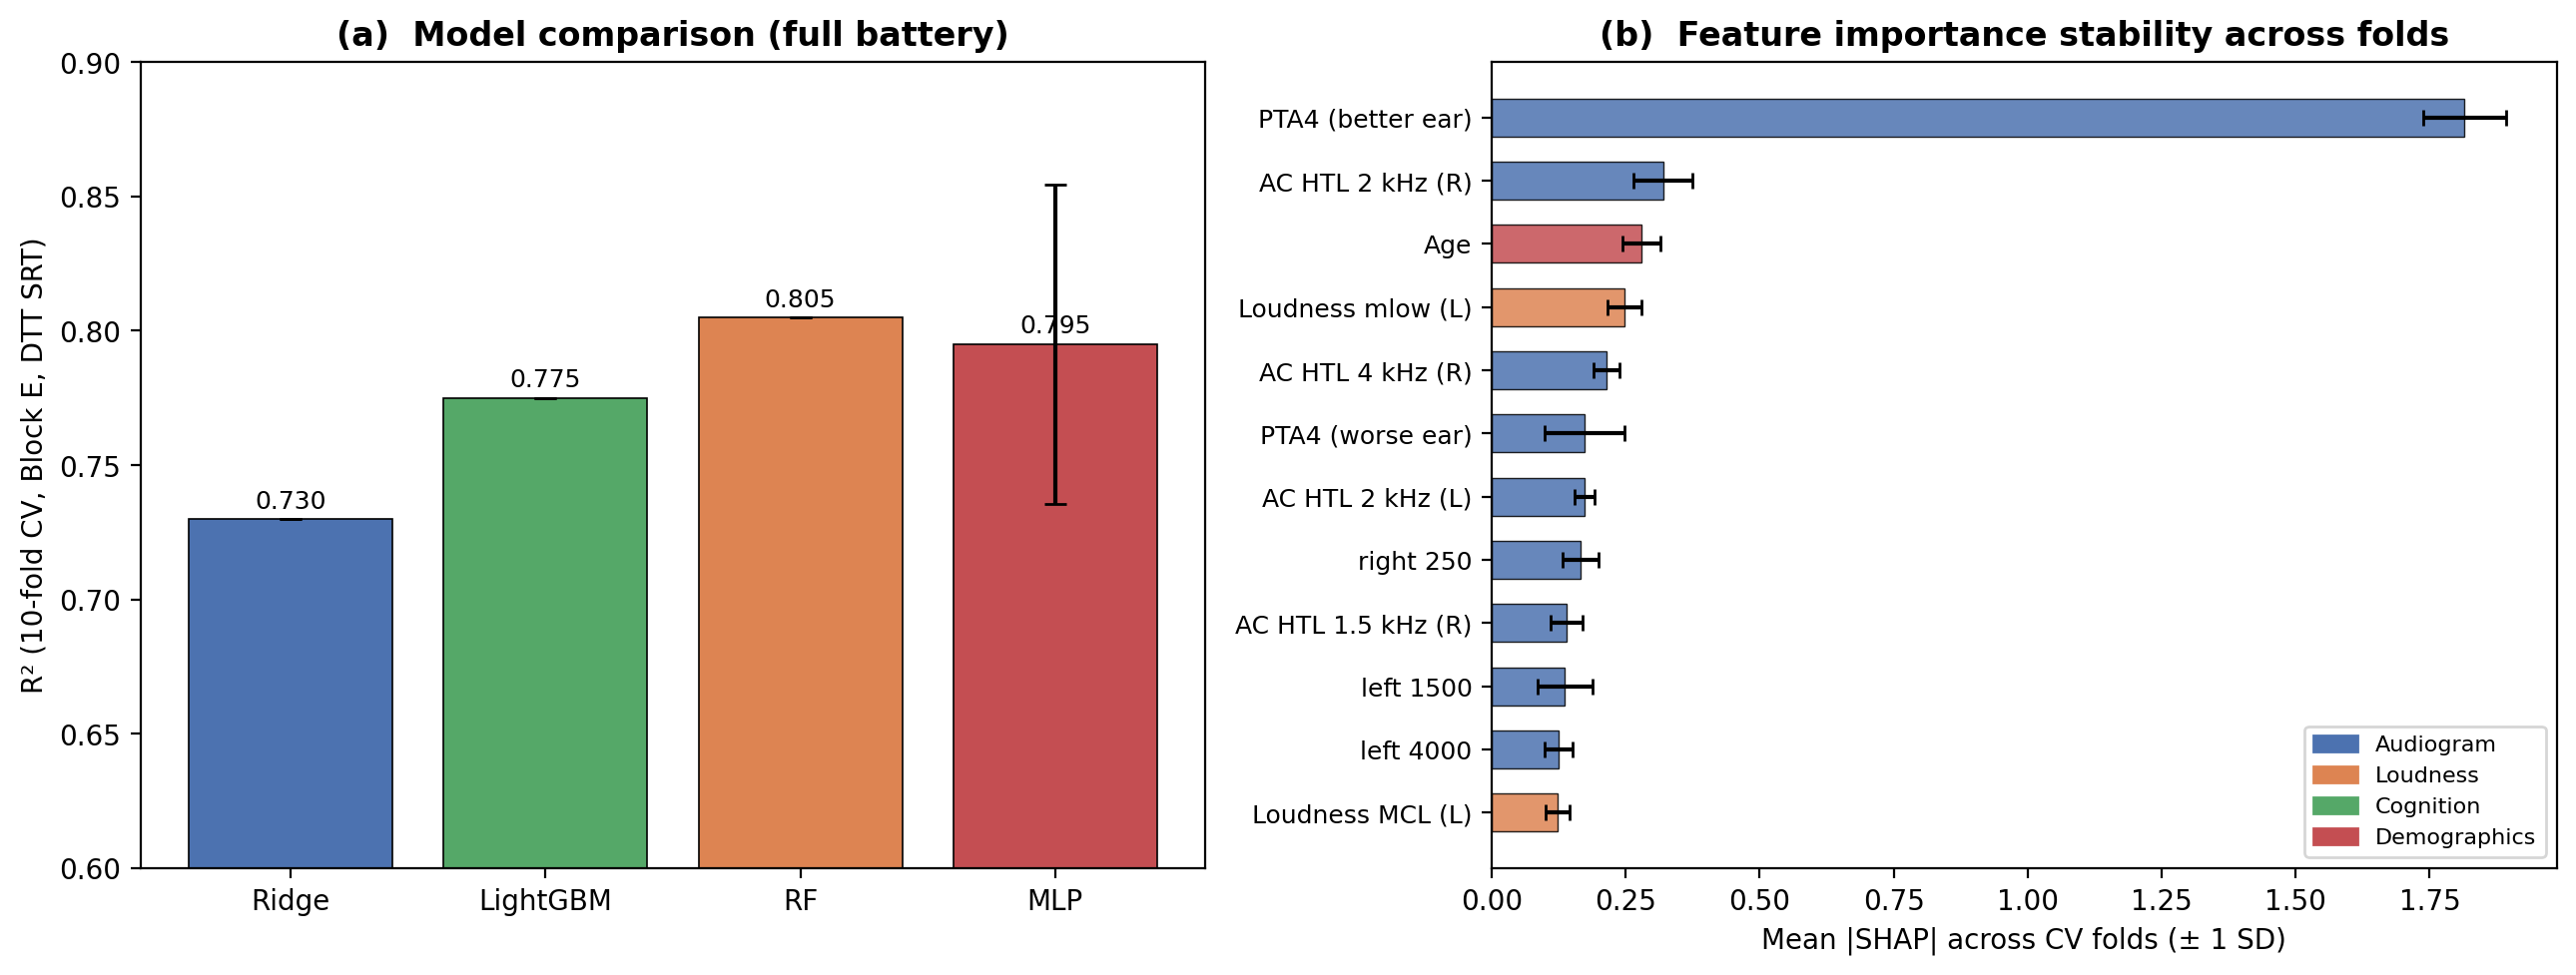
\includegraphics[width=0.95\textwidth]{fig6_model_comparison_stability.png}
  \caption{(a) DTT SRT $R^2$ (10-fold CV, Block~E) for Ridge, LightGBM,
  Random Forest, and MLP.  Tree ensembles and the MLP achieve similar
  performance; Ridge is consistently lower, suggesting non-linear structure
  in the feature--target relationship. (b) Mean absolute SHAP values
  (LightGBM, Block~E) with fold-level standard deviation bars.  Top-ranked
  features show low cross-fold variation (CV\,$<$\,0.15), confirming
  ranking stability.}
  \label{fig:comparison}
\end{figure*}

\begin{figure*}[t]
  \centering
  
\includegraphics[width=0.95\textwidth]{fig5_crosscohort.png}
  \caption{Cross-cohort validation: OHHR models applied to NHANES.
  (a) AUROC for predicting NHANES self-reported hearing difficulty (AUQ054)
  by feature set; adding age to PTA4 raises AUROC from 0.758 to 0.815.
  (b) Distribution of model-predicted P(poor SIN) stratified by NHANES
  AUQ054 category (1 = excellent, 5 = a lot of trouble, 6 = deaf); predicted
  risk increases monotonically with hearing difficulty category. (c) Calibration of PTA4-only and
  PTA4+Age classifiers evaluated on OHHR out-of-fold predictions.}
  \label{fig:crosscohort}
\end{figure*}

\end{document}
